\documentclass[12pt,a4paper,man,natbib]{apa6}

\usepackage[english]{babel}
\usepackage{times}
\usepackage[utf8x]{inputenc}
\usepackage{amsmath}
\usepackage{graphicx}
\usepackage[colorinlistoftodos]{todonotes}
\usepackage{subcaption}

\graphicspath{{figs/}}

\title{\large{Record Prediction Using Time Series Models}}
\author{Michael Rodgers}
\affiliation{SMGT 430, Rice University}
\shorttitle{Record Prediction Using Time Series Models}
\abstract{This paper uses Time Series models to 
predict a Major League Baseball team's final record. I 
explore several Time Series models and present the results. 
An advantage to the models explored in this paper is that 
they can generalize to any sport with minor changes. One 
sees that the best back-test was within an average of 5 
games error throughout 2005-2017. This is a fairly good 
result, considering that these models do not condition on 
annual team changes, but rather focus on the temporal 
structure of a team throughout its history.}
\authornote{Contact: mjr10@rice.edu \\ Date: April 20, 2018}
\keywords{Time Series, Sports Analytics, Record Prediction, 
MLB}

\begin{document}
\maketitle

I used data from the Lahman database for this project. There 
is an R package made by \cite{lahman} that I used to 
download the data. The Lahman data contains seasonal 
statistics. In order to predict a team's record, I modeled 
winning percentage using Time Series models. An assumption 
to use Time Series models is that the dependent variable is 
continuous and falls in the real line. In order to use this 
model, one must constrain the winning percentage interval to 
$[0, 1]$. This is done using the Transformation equation in 
Appendix C. This is a known technique used in logistic 
regression and is essential in this model.

\section{Methodology}

I present two results in the paper. One is the Mean Squared 
Prediction Error and the other is the 2018 record 
predictions. The MSPE allows one to understand how the model 
performed in the past. In order to accomplish this one needs 
to limit themselves to data that would have been available 
at the time. If one is trying to predict a team's 2017 
record, one can only use up to 2016 seasonal statistics. The 
2018 record predictions lets one see how the models forecast 
the future, but also gives insight into how the models 
typically predicted in the past. To perform this experiment, 
I used the R language. This back-test is accomplished using 
procedural programming, but I also made use of object-
oriented programming using the R6 package made by \cite{R6}. 
To fit the Time Series models, I used the forecast package 
made by \cite{forecast}.

\newpage

\section{Models}

The basis for all of these models is an ARIMA model. ARIMA 
stands for Autoregressive Integrated Moving Average model 
and is essentially linear regression on the past. Since 
we are modeling winning percentage, the independent features 
of the regression are winning percentage lagged by a certain 
value. For each model, I used the Maximum Likelihood 
Estimation for the coefficients. The models can be broken 
into two categories: base and ensemble learners. The base 
learners are BIC, PE and PYRIMA models, and the ensemble 
learners are naive and after weights models. 

\subsubsection{Bayesian Information Criteria (BIC)}

The BIC model uses the Bayesian Information Criteria to find 
the appropriate model for the Time Series. In the MSPE 
table, we see that it has the lowest average error; making 
it the best overall model.

\subsubsection{Pythagorean Expectation (PE)}

The PE model is known by most MLB analysts. We 
see that it performed the worst, but is not that far behind 
the statistical models. The PE model performs well for 
interpolation, but is not useful for predicting the future.

\subsubsection{Pythagorean Regressor (PYRIMA)}

The PYRIMA model does slightly better than the PE model, but 
some of the disadvantages of the PE equation are transfered 
into the Time Series model and cause it to perform poorly.

\subsubsection{Naive Weights}

The Naive Weights model performs slightly better than the 
After 2 model. This is probably because in addition to the 
regular terms, I also used seasonal terms in this model. So 
it used 16 models. This causes more aggregation, which leads 
to a better generalization. In the Naive Weights model, you 
give equal weight to each prediction. The After Weights 
model uses a technique to learn non-trivial weights.

\subsubsection{After Weights}

The After Weights models was inspired by \cite{after}. I 
changed the equation around a little to emphasize the 
training error more and introduced an alpha parameter. We 
see that the After 2 model performs better than the After 4 
model. After 4 used 16 models and the After 2 used 4 models. 
The After 4 model uses more complex models than the After 2 
and provides bias towards the more complex model weights. 
More complex models have a higher variance and are typically 
not robust. We this see in the results, but there are 
outliers.

\newpage

\section{Mean Squared Prediction Error (MSPE)}

The MSPE table allows for the models to be compared. We see 
that each team has a best model, so a team's predictions 
should be chosen based on how well a model performed in its 
back-test. This is something that an Information Criteria 
would not reveal. One sees a common trend that either single 
or aggregated forecasts perform better for a team. Since we 
are modeling winning percentage, all MSPE values are in 
measurements of percentages. We see that the lowest error 
was around 3\%, which translates to an error of 5 games.

\section{2018 Predictions}

The raw predictions give the predicted value and a 95\% 
confidence interval. This is useful because we can state 
that we are 95\% certain that a team's final record will be 
inside this interval. Unfortunately, this interval is so 
large that it is blatantly obvious that the final record 
will be inside these bounds. In order to draw inference in 
the raw predictions, I sorted the teams for each model by 
the amount of wins. This allows each team to be ranked and 
lets one see how balanced the teams will be with regards to 
who is over and under .500. 

\section{Conclusion and Future Study}

Time Series modeling is a tool that provides decent results 
and limits the complexity of the model. One of the key 
attributes of Time Series models is that they can model 
anything that revolves around time, so this technique can be 
used for any sport, not just baseball. To increase the 
accuracy, one needs to factor in team annual changes. This 
would be useful since a team can improve dramatically over 
two seasons if they are in a rebuilding stage.

\bibliography{references}

\appendix

\section{MSPE from 2005-2017}

\begin{figure}
\begin{center}
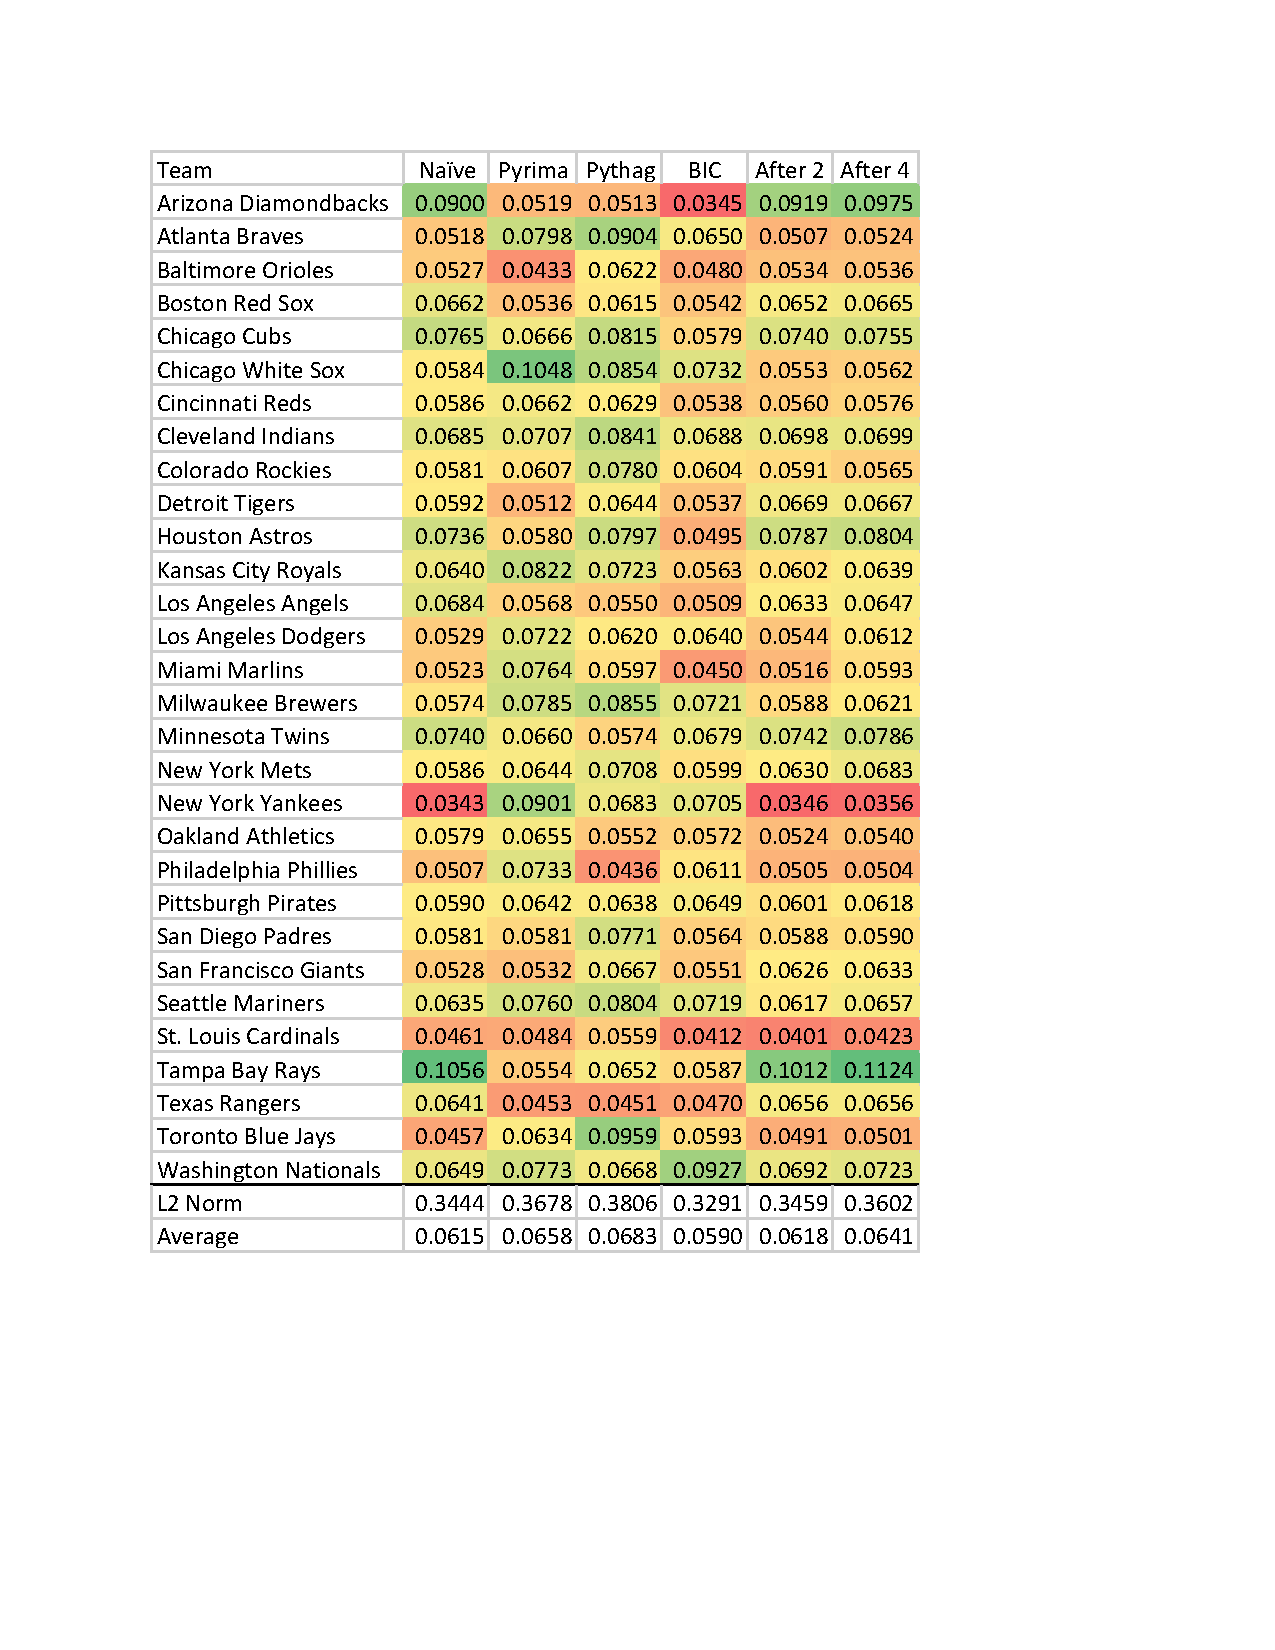
\includegraphics[width = 5in]{mspe.pdf}
\caption{MSPE}
\label{fig:MSPE}
\end{center}
\end{figure}

\section{2018 Predictions}

\subsection{Raw}

\begin{figure}
\begin{center}
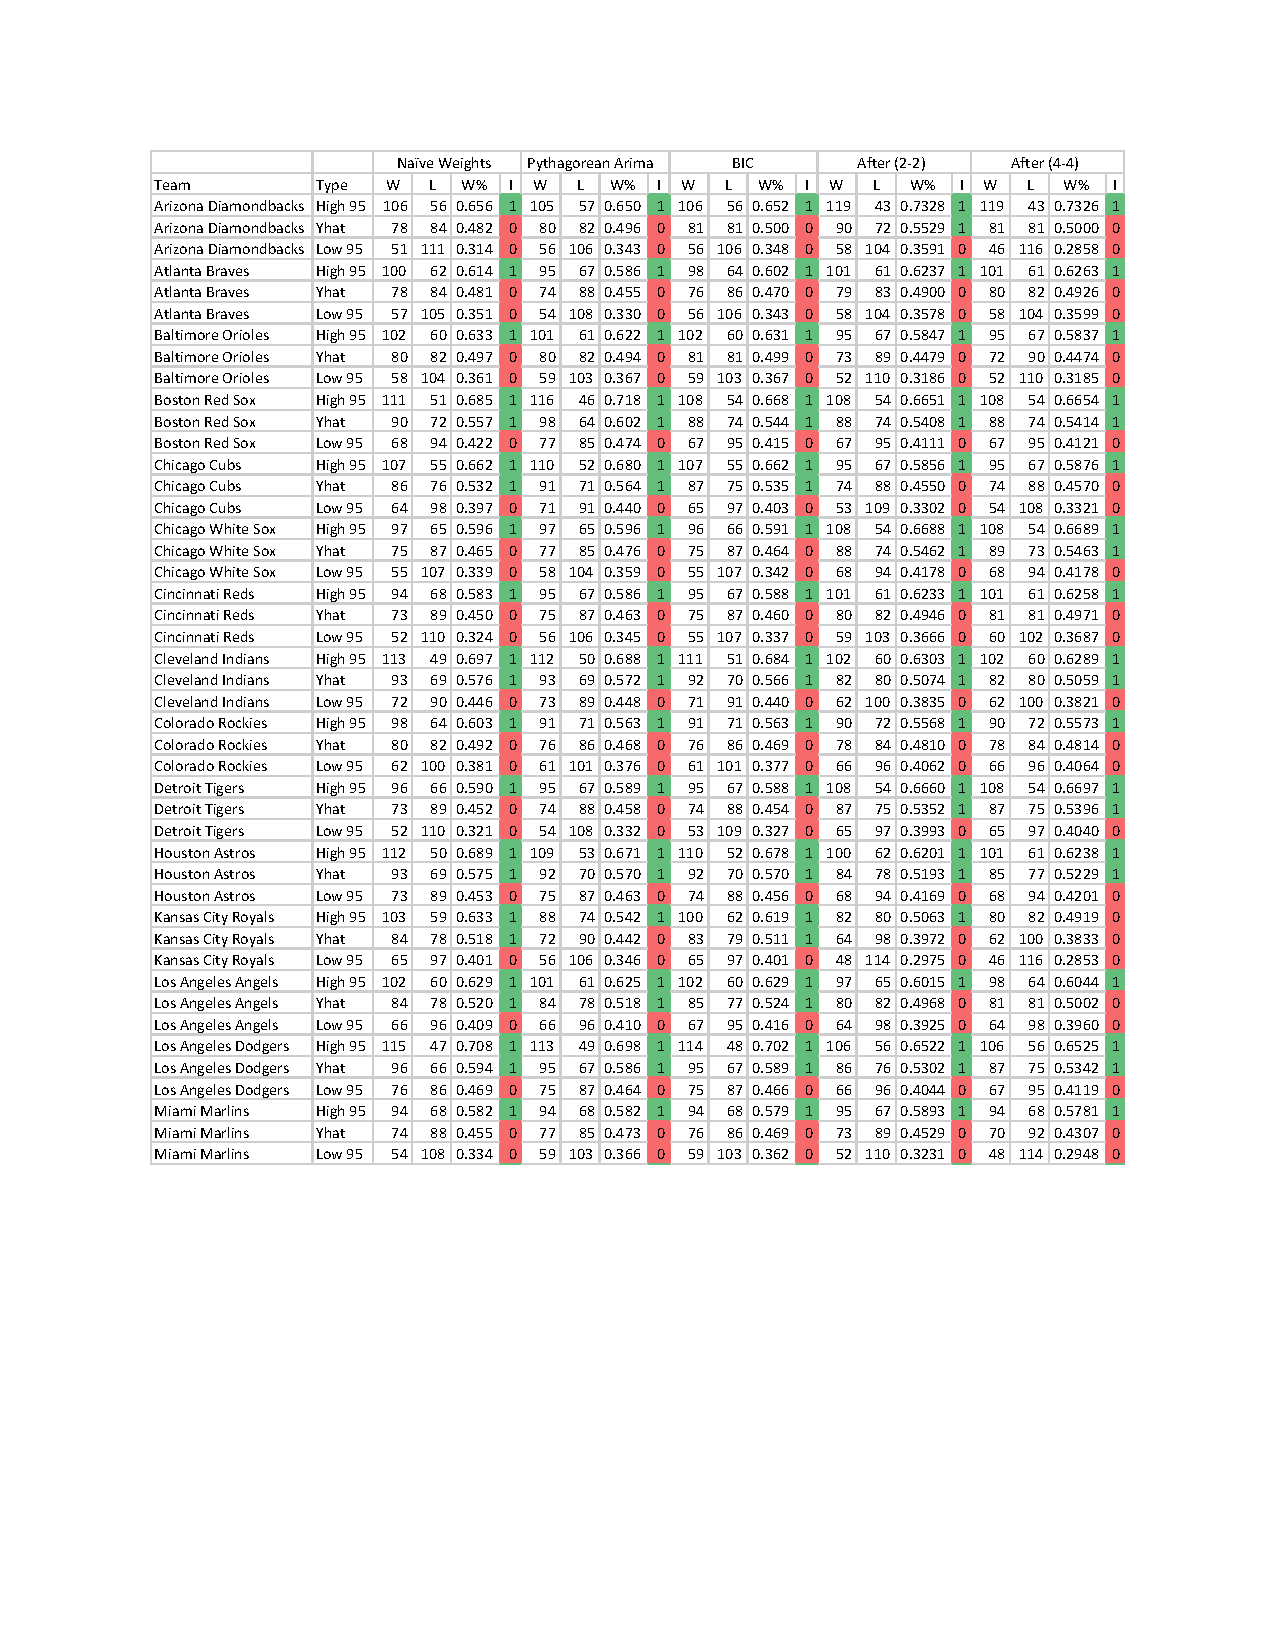
\includegraphics[width = 6in]{2018_top.pdf}
\caption{Raw 1-15}
\label{fig:Raw 1-15}
\end{center}
\end{figure}

\newpage

\begin{figure}
\begin{center}
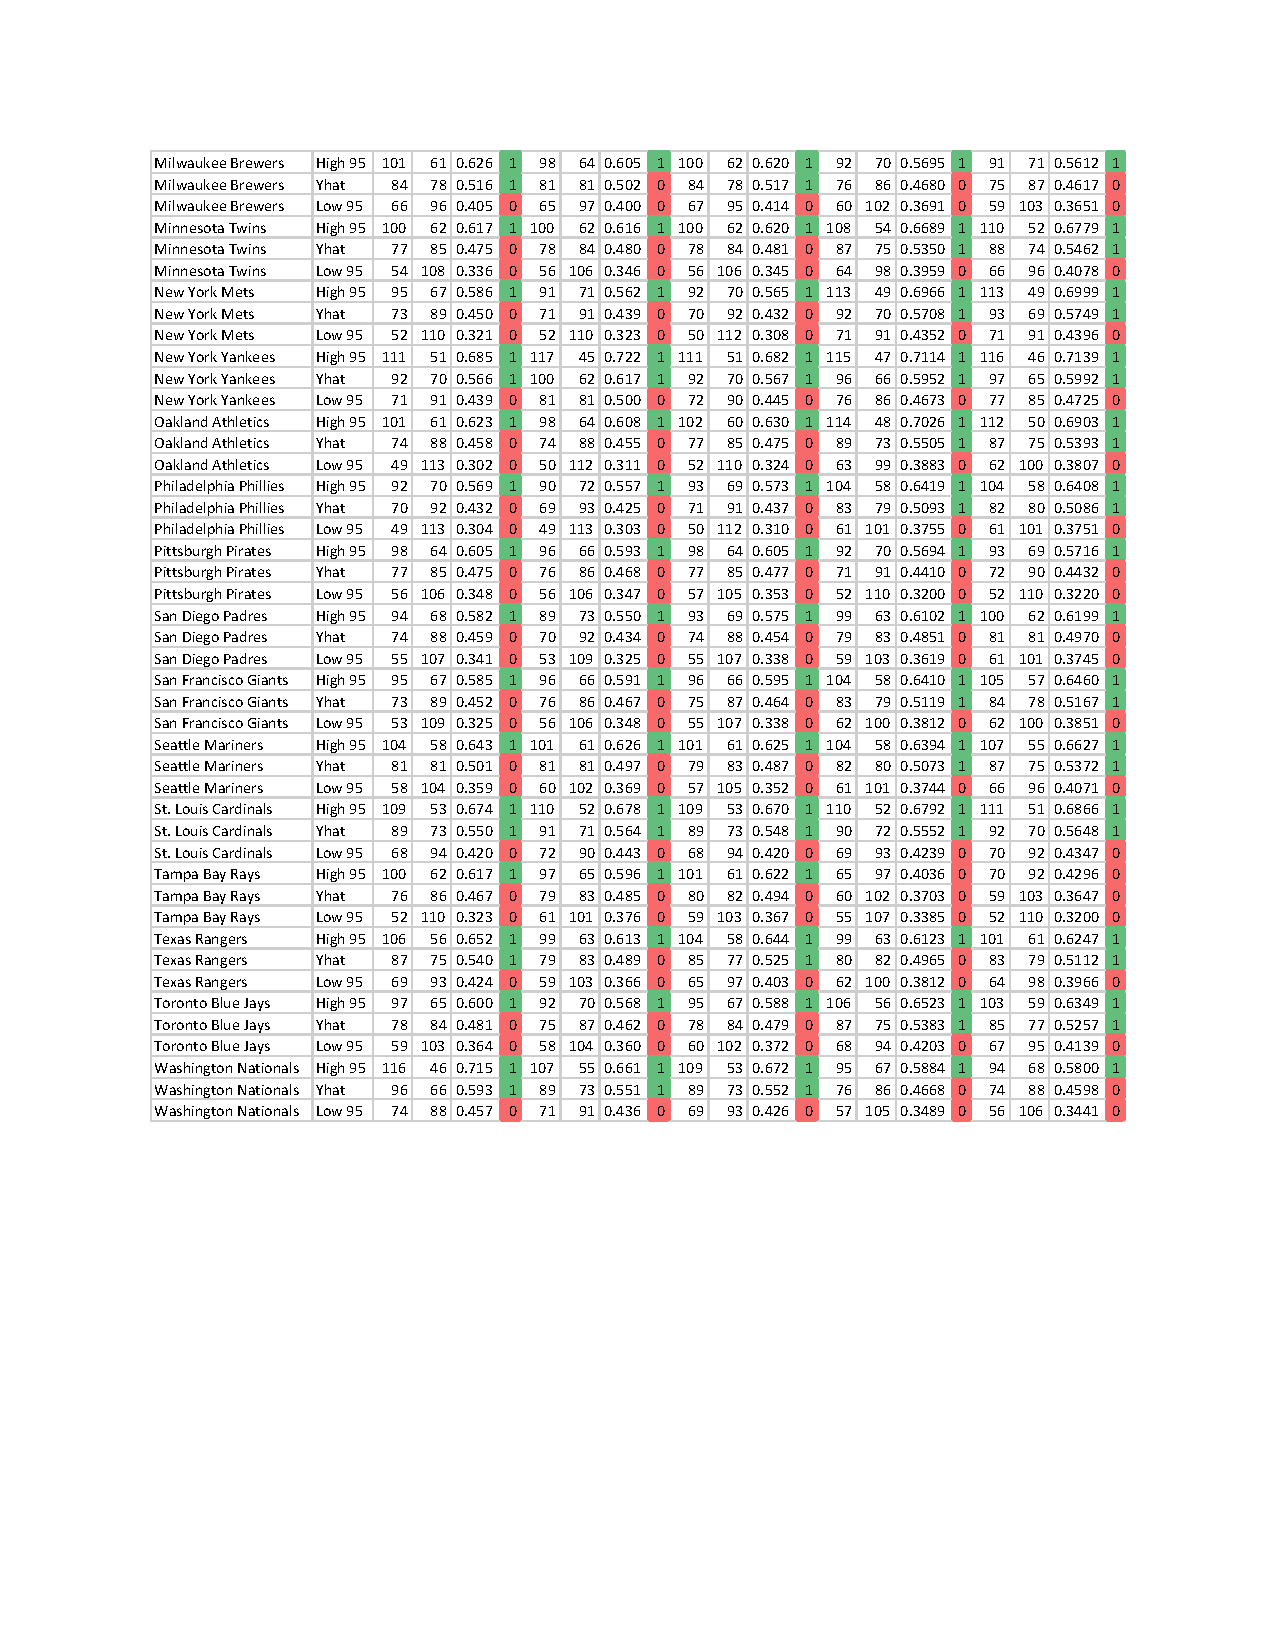
\includegraphics[width = 6in]{2018_bottom.pdf}
\caption{Raw 16-30}
\label{fig:Raw 16-30}
\end{center}
\end{figure}

\newpage

\subsection{Ranked}

\newcommand{\rankedwidth}{13cm}

\begin{figure}
\begin{center}
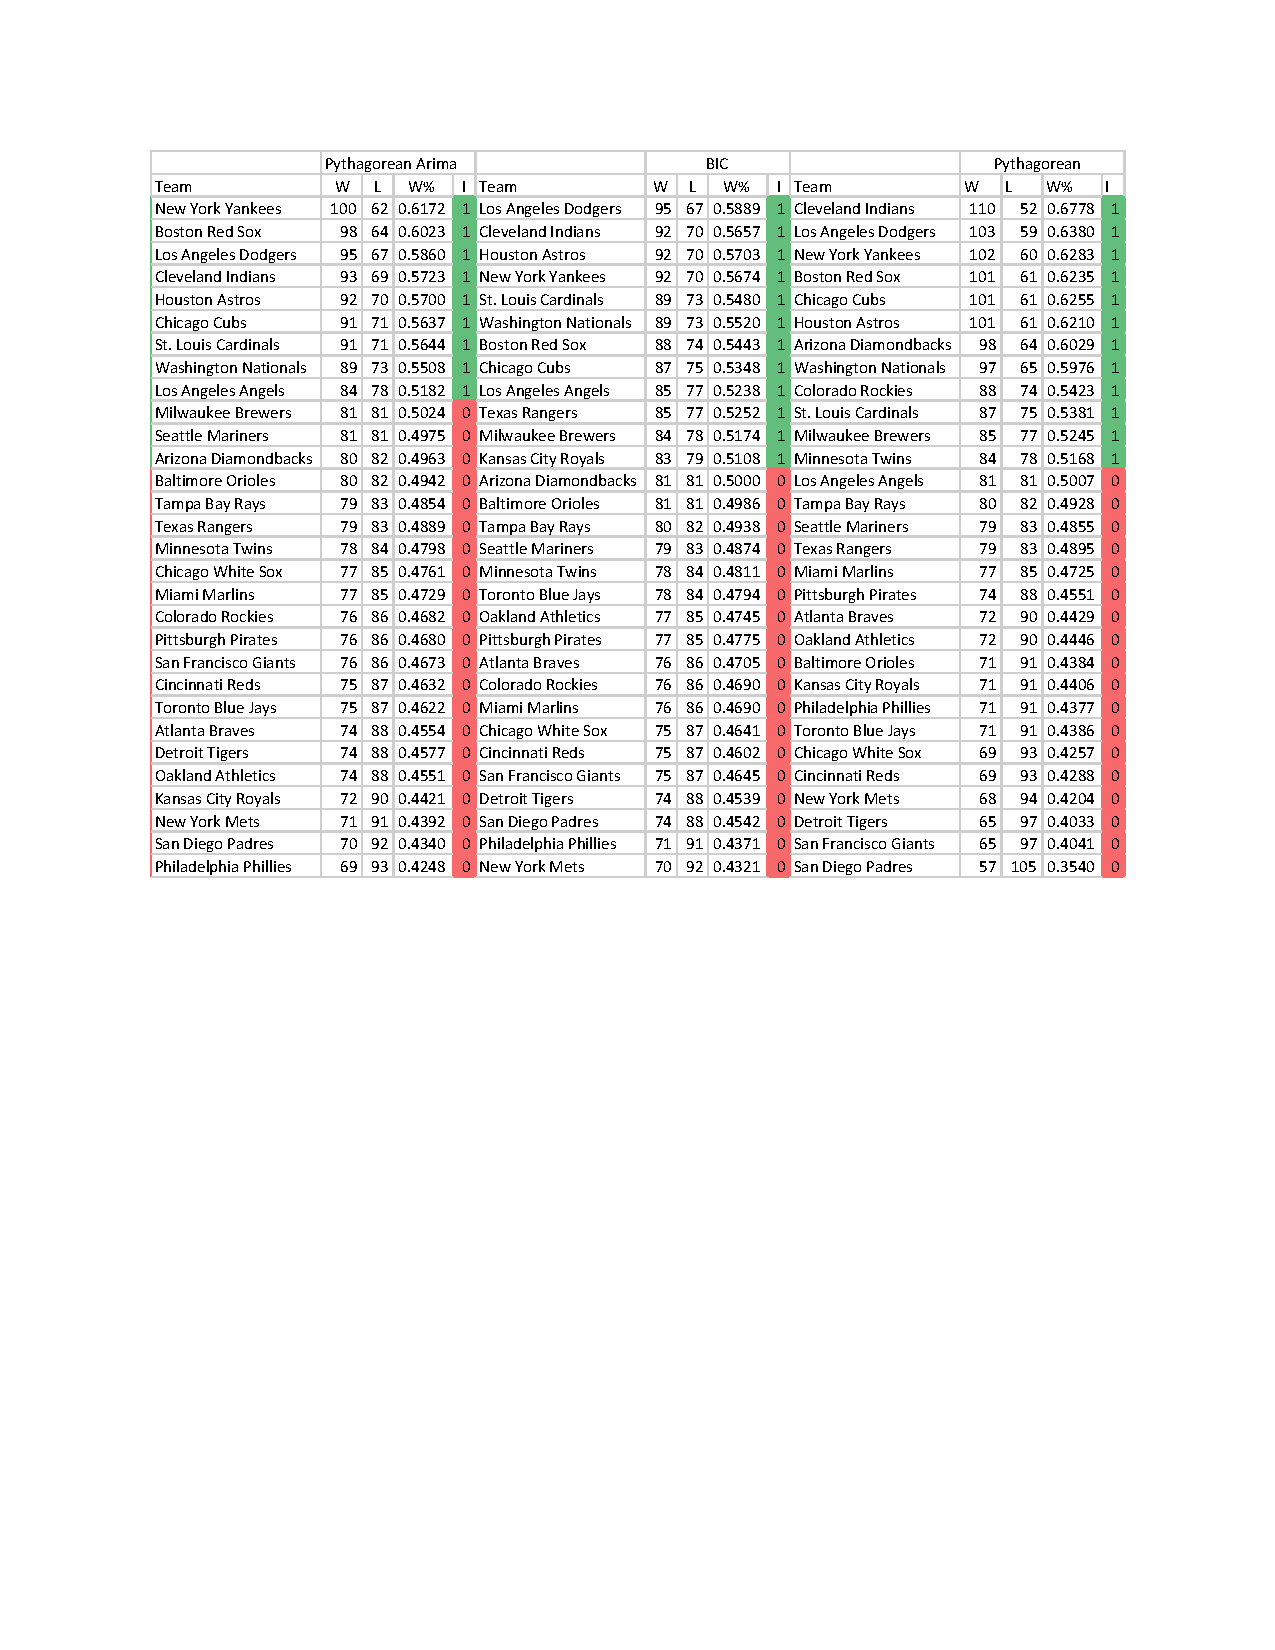
\includegraphics[width = \rankedwidth]{2018_ranked_top.pdf}
\caption{Ranked 1-15}
\label{fig:Ranked 1-15}
\end{center}
\begin{center}
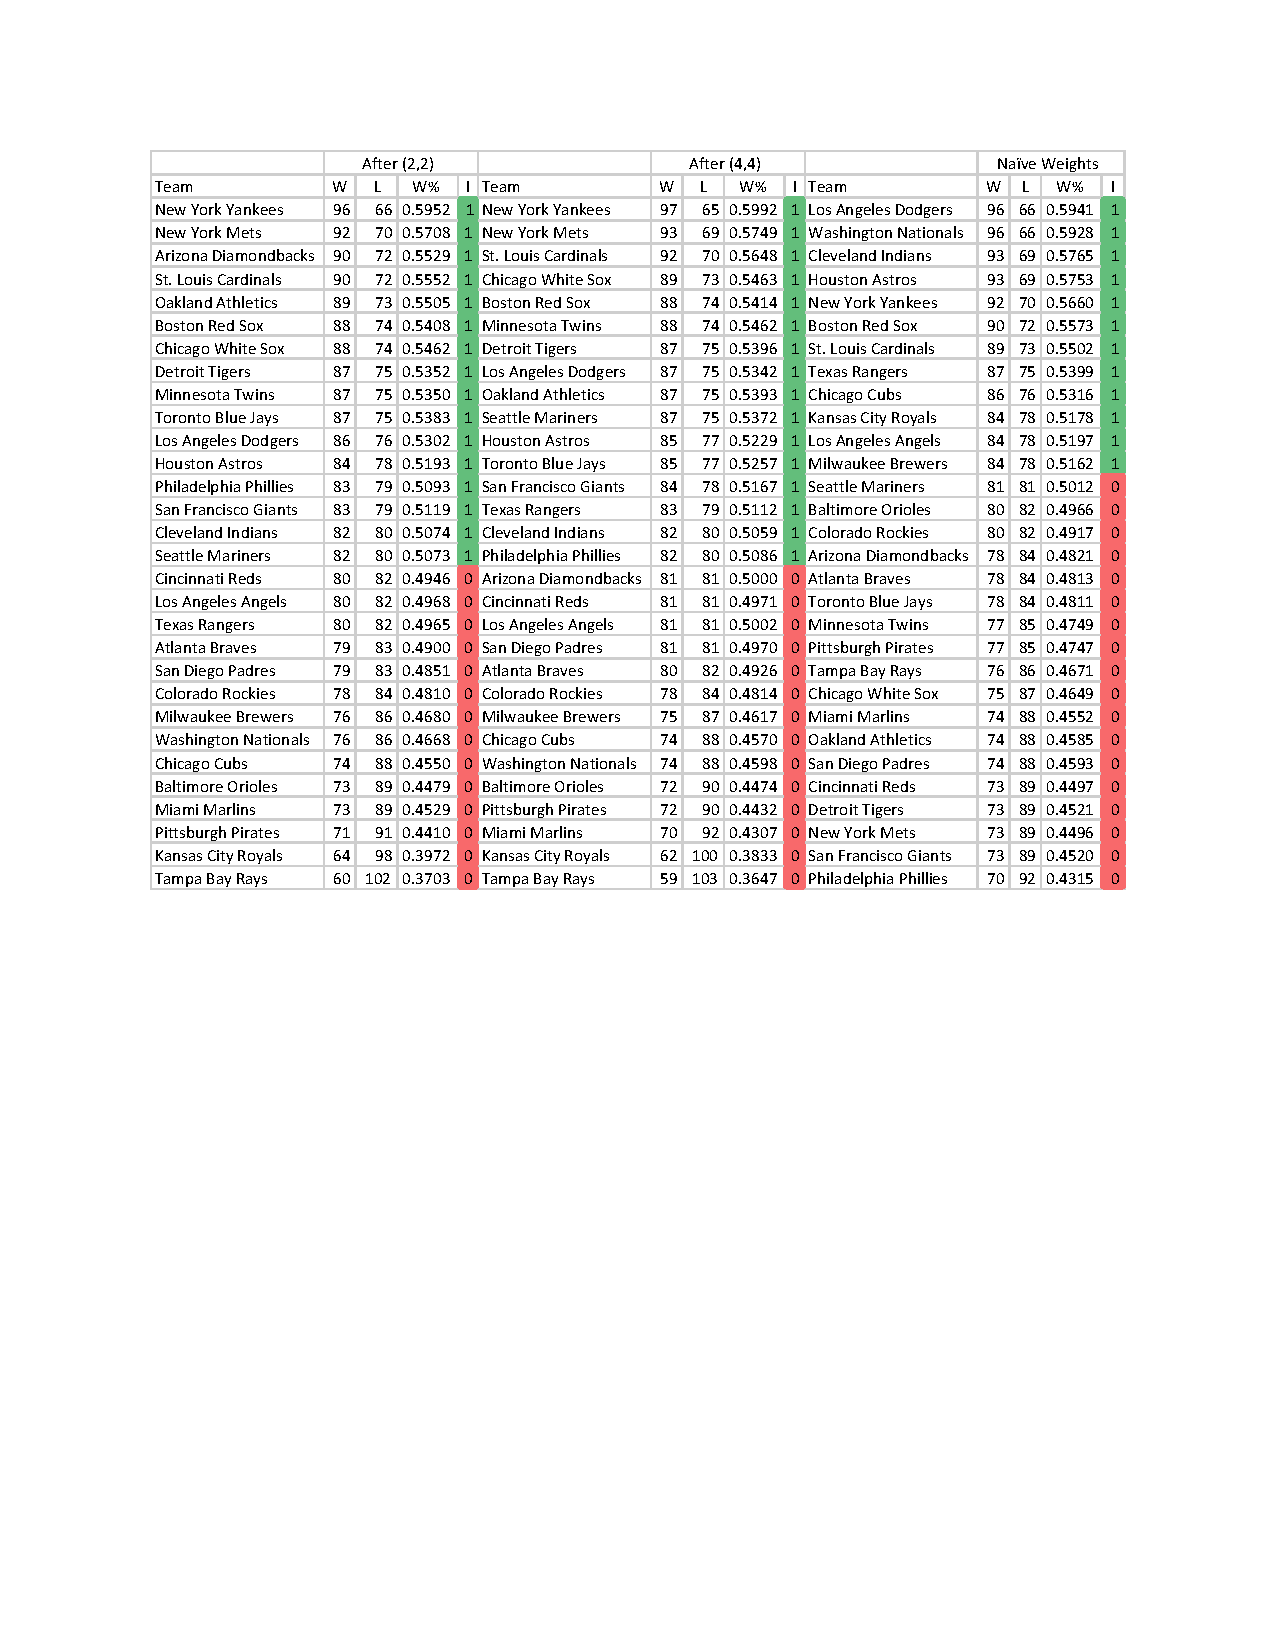
\includegraphics[width = \rankedwidth]
{2018_ranked_bottom.pdf}
\caption{Ranked 16-30}
\label{fig:Ranked 16-30}
\end{center}
\end{figure}

\section{Equations}

\subsection{Mean Squared Prediction Error (MSPE)}

$$
\text{MSPE} = \sqrt{\frac{\sum_{i=1}^{n} (y_i - \hat{y}_i)^2}{n}}
$$

\subsection{Transformation}

$$
W'_t = \log(\frac{W_t}{1-W_t})
$$
$$
W_t^{-1} = \frac{1}{e^{-W'_t} + 1}
$$

\subsection{Arima(p, d, q)}
$$ 
Y_t = (1-B)^d W'_t 
$$
$$ 
(1 - \sum_{i=1}^{p} \phi_i B^i) Y_t = 
(1 + \sum_{i=1}^{q} \theta_i B^i) \epsilon_t
$$

\subsection{Bayesian Information Criteria (BIC)}
$$
W'_t = Arima(BIC)
$$

\subsection{Pythagorean Expectation}
$$
W_t = P_{t-1} = \frac{RS_{t-1}^2}{RS_{t-1}^2 + RA_{t-1}^2}
$$

\subsection{Pyrima}
$$
W'_t = Arima(BIC) + \beta P_{t-1}
$$

\subsection{Naive Weights}
$$
W'_t = \frac{\sum_{i=1}^p \sum_{j=1}^q Arima(i, d, j)}{p*q}
$$

\subsection{After Weights}
$$
\lambda_{m, t=1} = \frac{1}{M}
$$
$$
\lambda_{m, t\geq2} = 
\frac
{
\prod_{i=1}^{n-1} e^{\frac{-\alpha}{n_{\text{tr}, i}} 
\sum_{j=1}^{n_{\text{tr}, i}} W_{j,i}-\hat{W}_{j,i}}
}
{
\sum_{m=1}^{M}
\prod_{i=1}^{n-1} e^{\frac{-\alpha}{n_{\text{tr}, i}} 
\sum_{j=1}^{n_{\text{tr}, i}} W_{j,i}-\hat{W}_{j,i}}
}
$$

$$
W'_{t} = \sum_{i=1}^{M} \lambda_{i, t} \hat{W}_{t,i}
$$

\end{document}
